%設定頁面
\documentclass[12pt,a4paper]{article}
\usepackage[margin=1in,a4paper]{geometry}

%設定中文
\usepackage{xeCJK} 
\setCJKmainfont{標楷體} 
\XeTeXlinebreaklocale "zh"   
\XeTeXlinebreakskip = 0pt plus 1pt 

%浮水印
%\usepackage{draftwatermark}
%\SetWatermarkText{\bf NTNU MATH}
%\SetWatermarkScale{0.7}

%圖片
\usepackage{graphicx}
\usepackage{subfigure}

%頁首頁尾
\makeatother
\usepackage{fancyhdr}

%顏色
\usepackage{xcolor}

%表格顏色
\usepackage{colortbl}

%設定數學
\usepackage{amsmath, amsthm, amssymb}
\makeatletter

%自定圈圈標號
\usepackage{pstricks,pstricks-add}
\newcommand\textc[1]{{\begin{pspicture*}
(-0.25,-0.2)(0.25,0.3)\rput[c](0,0)
{\large \textcircled{\footnotesize #1}}
\end{pspicture*} }}

%自訂向量符號
\def\leftharpoonfill@{\arrowfill@\leftharpoonup\relbar\relbar}
\def\rightharpoonfill@{\arrowfill@\relbar\relbar\rightharpoonup}
\newcommand\rbjt{\mathpalette{\overarrow@\rightharpoonfill@}}
\newcommand\lbjt{\mathpalette{\overarrow@\leftharpoonfill@}}

%自訂定理
\newtheorem*{thm}{Theorem}
\newtheorem*{lem}{Lemma}
\newtheorem*{de}{Definition}
\newtheorem*{rmk}{Remark}
\newtheorem*{ex}{Example}
\newtheorem*{pf}{Proof}
\newtheorem*{sol}{Solution}

%程式碼
\usepackage{listings}
\usepackage{color}

\definecolor{dkgreen}{rgb}{0,0.6,0}
\definecolor{gray}{rgb}{0.5,0.5,0.5}
\definecolor{mauve}{rgb}{0.58,0,0.82}

\lstset{
  basicstyle={\small \ttfamily},
  frame=tb,
  language=Python,
  aboveskip=3mm,
  belowskip=3mm,
  showstringspaces=false,
  columns=flexible,
  basicstyle={\small\ttfamily},
  numbers=left,
  numbersep = 14pt,
  numberstyle=\tiny\color{gray},
  keywordstyle=\color{blue},
  commentstyle=\color{dkgreen},
  stringstyle=\color{mauve},
  breaklines=true,
  breakatwhitespace=true,
  tabsize=3,
  backgroundcolor=\color{gray!10}
}




%作者
\title{NTNU影像處理HW12}
\author{廖家緯}
\date{2020.6.4}

\begin{document}
\maketitle
%標題、作者、日期
\fontsize{12pt}{20pt}\selectfont
%設定字體大小、間距
\setlength{\baselineskip}{20pt}
%設定行距

\pagestyle{fancy}
\lhead{}
\chead{}
\rhead{}
\lfoot{}
\cfoot{\thepage}
\rfoot{}
\renewcommand{\headrulewidth}{0pt} %上線寬
\renewcommand{\footrulewidth}{0pt} %下線寬
%\renewcommand{\abstractname}{Executive Summary}




%正文開始
\begin{enumerate}
\item[•]{\bf Outline}:\\
Implement the Lantuejoul's skeletonization method 
using the structuring element
\begin{center}
\begin{tabular}{cc}
\begin{tabular}{|c|c|c|}
\hline
 & $\bullet$ &\\
\hline
$\bullet$ & $\bullet$ & $\bullet$\\
\hline
 & $\bullet$ &\\
\hline
\end{tabular}
&
\begin{tabular}{|c|c|c|}
\hline
$\bullet$ & $\bullet$ & $\bullet$\\
\hline
$\bullet$ & $\bullet$ & $\bullet$\\
\hline
$\bullet$ & $\bullet$ & $\bullet$\\
\hline
\end{tabular}\\
Cross $(B_1)$ & Square $(B_2)$
\end{tabular}
\end{center}




Apply the method to the following input image.\\


\item[•]
{\bf Code(Python):}
\begin{lstlisting}
# coding: utf-8
import numpy as np
import cv2

#轉成二值影像
def binary_img(I):
    I_ = I.copy()
    for i in range(n):
        for j in range(m):
            if I[i][j] > 128:
                I_[i][j] = 1
            else:
                I_[i][j] = 0
    return I_

#Lantuejoul’s method
def Lantuejouls_method(I, B):
    I_ = I.copy()
    Erosion = np.zeros((n, m)).astype('uint8')
    Opening = np.zeros((n, m)).astype('uint8')
    Differences = np.zeros((n, m)).astype('uint8')
    Union = np.zeros((n, m)).astype('uint8')
    k = 0

    while k < 50:
        for i in range(1, n-1):
            for j in range(1, m-1):
                if np.array_equal(I_[i-1:i+2, j-1:j+2]*B, B):
                    Erosion[i][j] = 1

        for i in range(1, n-1):
            for j in range(1, m-1):
                if Erosion[i][j] == 1:
                    Opening[i-1:i+2, j-1:j+2] = np.ones(3)

        Differences = I_ - Opening
        Union = Union + Differences
        k += 1
        if np.array_equal(Opening, np.zeros((n, m))):
            break
        else:
            I_ = Erosion
            Erosion = np.zeros((n, m)).astype('uint8')
            Opening = np.zeros((n, m)).astype('uint8')
            
    Union = (Union*255).astype('uint8')
    return Union

# 顯示圖片
def imgshow(img):
    cv2.imshow('My Image', img)
    cv2.waitKey(0)
    cv2.destroyAllWindows()

I = cv2.imread('img.png', cv2.IMREAD_GRAYSCALE)
n, m = np.shape(I)

B1 = np.array([[0, 1, 0], [1, 1, 1], [0, 1, 0]]).astype('uint8')
B2 = np.array([[1, 1, 1], [1, 1, 1], [1, 1, 1]])

I1 = binary_img(I)
I1 = Lantuejouls_method(I1, B1)
imgshow(I1)
cv2.imwrite('4-connected components.jpg', I1)

I2 = binary_img(I)
I2 = Lantuejouls_method(I2, B2)
imgshow(I2)
cv2.imwrite('8-connected components.jpg', I2)

\end{lstlisting}

\newpage
\item[•]
{\bf Input image:}\\
\begin{figure}[h]
\hspace*{12em}
\begin{tabular}{c}

\includegraphics[height=2.5in]{img.png}\\
Input image
\end{tabular}
\end{figure}

\item[•]
{\bf Result:}
\begin{figure}[h]
\hspace*{5em}
\begin{tabular}{cc}
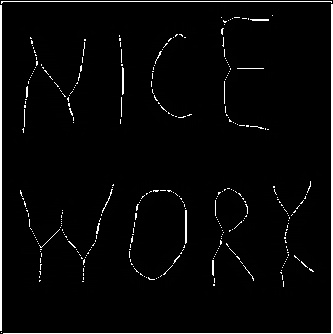
\includegraphics[height=2.5in]
{4-connected components.jpg}&
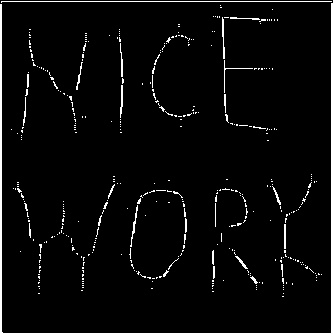
\includegraphics[height=2.5in]
{8-connected components.jpg}\\
4-connected components & 8-connected components
\end{tabular}
\end{figure}


\item[•]
{\bf Experience:}\\
這次作業一開始寫的code時間複雜度超過$O(n^4)$,程式跑超久,後來和同學討論後砍掉重練,調整方法,並不斷優化,寫出這次作業。而我怕$k$值太大,導致程式執行時間超級久,因此我在迴圈上設了$k<50$,一般而言,執行差不多$50$次,已經可呈現效果。
\end{enumerate}










\end{document}